%%=============================================================================
%% Push-notificaties
%%=============================================================================

\chapter{Notificaties}%
\label{ch:notificaties}

In dit hoofdstuk gaan we de lokale notificaties van native en cross-platform vergelijken. 
Met deze resultaten kunnen we dan een gepaste conclusie vormen.

\section{Native}
\subsubsection{Wat hebben we nodig}
Om lokale notificaties aan te kunnen maken bij Android maken we gebruik van de NotificationCompat API aangeboden 
door de Android support library. Deze stelt ons in staat om de titel, tekst, pictogram en andere inhoud van de 
notificatie in te stellen. Notificaties kunnen ook worden ingesteld om speciale acties te ondernemen bij het openen 
van de applicatie via de notificatie. Er kan ook een eventueel een prioriteit worden meegegeven.

\subsubsection{Uitvoering}
\paragraph{1. Dependancy toevoegen}
Normaal zijn bevatten alle projecten gestart met Android Studio de nodige dependancies om de NotificationCompat API
te gebruiken. Maar voor de zekerheid verifiëren we dat onderstaande dependancy er bij zit.
\begin{minted}{java}
  val core_version = "1.6.0"
  dependencies {
      implementation("androidx.core:core-ktx:$core_version")
  }
\end{minted}
Als de dependancy is toegevoegd dan kunnen we notificaties beginnen aanmaken.

\paragraph{2. Notificatie aanmaken}
Om een notificatie aan te maken gaan we het NotificationCompat.Builder object gebruiken. 
\begin{minted}{kotlin}
   var builder = NotificationCompat.Builder(this, CHANNEL_ID)
    .setSmallIcon(DRAWABLE_ICON)
    .setContentTitle(TITLE)
    .setContentText(DESCRIPTION)
    .setPriority(NotificationCompat.PRIORITY_DEFAULT)
\end{minted}
\begin{figure}[H]
    \centering
    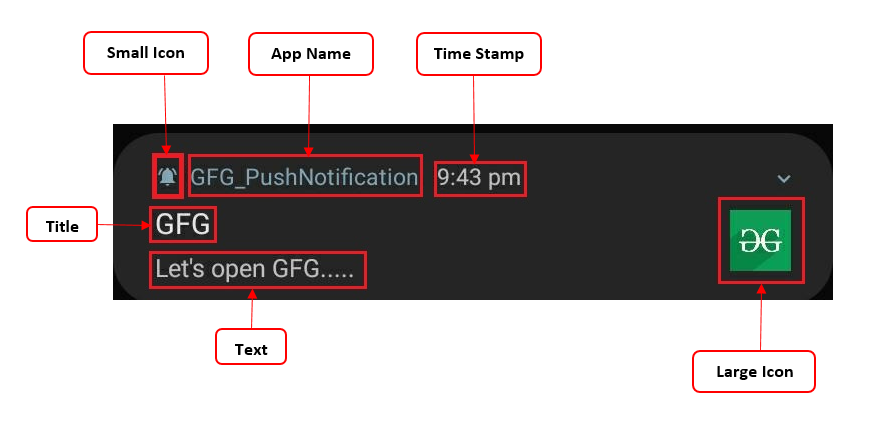
\includegraphics[height=0.2\textheight]{NotificationAnatomy.png}
    \caption{Anatomy standaard notificatie .}% TODO \parencite{https://www.geeksforgeeks.org/how-to-push-notification-in-android/}
\end{figure}

\paragraph{3. Channel aanmaken}
Het laatste dat we nodig hebben vooraleer de notificatie getoond kan worden is een channel. Deze worden 
gebruikt om notificaties te groeperen volgens hun belang. Om een channel aan te maken gebruiken we 
de .createNotificationChannel() methode. Het maakt niet uit wanneer of waar deze code wordt uitgevoerd. 
Het is enkel belangrijk dat de channel wordt aangemaakt vooraleer er wordt geprobeerd om notificaties 
te tonen. Dus best zo vroeg mogelijk in de applicatie.
\begin{minted}{kotlin}
private fun createNotificationChannel() {
  // Channel aanmaken
  val channel = NotificationChannel(CHANNEL_ID, CHANNEL_NAME, 
        NotificationManager.IMPORTANCE_DEFAULT).apply {
    description = CHANNEL_DESCRIPTION
  }
  // Channel bij het systeem registreren
  val notificationManager: NotificationManager =
    getSystemService(Context.NOTIFICATION_SERVICE) as NotificationManager
  notificationManager.createNotificationChannel(channel)
}
\end{minted}

\paragraph{4. Actie toevoegen}
Als onderdeel van de performantie te testen, zullen we de notificaties instellen om niet het hoofdscherm, 
maar een ander scherm te tonen bij het openen van de applicatie via de notificatie. Dit kunnen we doen met 
de Intent en PendingIntent objecten. Aan het Intent object kunnen acties worden meegegeven. Hier wordt er 
gespecificeerd welk scherm en welke actie er moet gebeuren. Daarna wordt het Intent object aan het PendingIntent 
object meegegeven dat op zijn beurt wordt meegegeven aan de .setContentIntent(PENDINGINTENT) methode.
\begin{minted}{kotlin}
  Intent intent = new Intent(context, SpecifiekSchermActivity.class);
  intent.setAction("ACTION_MY_ACTION");
  PendingIntent pendingIntent = PendingIntent.getActivity(context, 0, 
    intent, PendingIntent.FLAG_UPDATE_CURRENT);

  var builder = NotificationCompat.Builder(this, CHANNEL_ID)
    .setSmallIcon(DRAWABLE_ICON)
    .setContentTitle(TITLE)
    .setContentText(DESCRIPTION)
    .setPriority(NotificationCompat.PRIORITY_DEFAULT)
    .setContentIntent(pendingIntent) // Voeg deze toe
\end{minted}

\paragraph{5. Notificatie tonen}
Tot slot kunnen we dan de notificatie tonen met de .notify() methode van de NotificationManagerCompat. 
Eerst wordt de notificationManager aangemaakt waarna de notificatie wordt getoond.
\begin{minted}{kotlin}
  NotificationManagerCompat notificationManager = 
    NotificationManagerCompat.from(context);
  notificationManager.notify(notificationId, builder.build());
\end{minted}

\subsubsection{Ontwikkeltijd}

\paragraph{Geïnvesteerde tijd}

\paragraph{Compiletijd}

\subsubsection{Performantie}

\subsubsection{Schaalbaarheid}

\subsubsection{Conclusie}


\section{Cross-platform}
\subsubsection{Wat hebben we nodig}
Om lokale notificaties bij React native te tonen gaan we gebruik maken van de externe library Notifee.
Met deze library kunnen we net zoals bij Android de notificatie aanpassen naar onze wensen.

\subsubsection{Uitvoering}
\paragraph{1. Library toevoegen}
Als eerst voegen we Notifee toe aan de root van ons project.
\begin{minted}{bash}
  npm install --save @notifee/react-native
\end{minted}
Nu kunnen we de library importeren in de bestanden waar we deze nodig hebben.
\begin{minted}{typescript}
  import notifee from '@notifee/react-native';
\end{minted}

\paragraph{2. Toestemming vragen \& channel aanmaken}
Nog voor we een notificatie kunnen tonen moeten we eerst de toestemming vragen aangezien dit bij React native 
niet automatisch gebeurt zoals bij Android Studio. Ook moeten we net zoals bij Android Studio 
een channel aanmaken om de notificaties te groeperen. Het maakt niet uit wanneer dit gebeurt, maar 
het moet wel gebeuren voor er een notificatie wordt getoond. Dus best zo vroeg mogelijk in de applicatie.
\begin{minted}{typescript}
  await notifee.requestPermission()

  const channelId = await notifee.createChannel({
    id: 'default',
    name: 'Default Channel',
  });
\end{minted}

\paragraph{3. Notificatie aanmaken}
Bij React native wordt de notificatie ook direct getoond bij het maken ervan. Net zoals bij Android Studio 
geven we de naam, description, channelId en optioneel een icon (default ic\_launcher). 
\begin{minted}{typescript}
  await notifee.displayNotification({
    title: 'TITLE',
    body: 'DESCRIPTION',
    android: {
      CHANNEL_ID,
      smallIcon: ICON_NAME,
      pressAction: {
        id: 'default',
      }, // Zorgt ervoor dat de applicatie opent 
         // bij het drukken op de notificatie
    },
  });
\end{minted}

\paragraph{4. Actie toevoegen}
Zoals besproken bij native zullen we niet het homescherm openen als we op een notificatie drukken maar zullen we 
direct naar een ander scherm navigeren. Hiervoor hebben we nog een extra library nodig namelijk \textbf{@react-navigation/native}. 
\subparagraph{1. Library toevoegen} 
Voeg de navigatie library toe aan de root van ons project
\begin{minted}{bash}
  npm install @react-navigation/native
  npm install react-native-screens react-native-safe-area-context
\end{minted}

\subparagraph{2. Android configuratie} % TODO path naar mainactivity
Voeg de onCreate methode toe aan de MainActivity.
\begin{minted}{java}
  public class MainActivity extends ReactActivity {
    // ...
    @Override
    protected void onCreate(Bundle savedInstanceState) {
      super.onCreate(null);
    }
    // ...
  }
\end{minted}
Om dan te detecteren wanneer er op een notificatie wordt gedrukt maken we gebruik van EVENTS. Er is een onForegroundEvent 
dat wordt geroepen indien de applicatie open staat. Als dit niet het geval is, wordt de onBackgroundEvent 
aangeroepen. Deze EVENTS kunnen gebruikt worden om dan naar een scherm te navigeren indien de applicatie geopend wordt.
\begin{minted}{typescript}
  import { useNavigation } from '@react-navigation/native';

  const navigation = useNavigation();

  notifee.onForegroundEvent(({ type, detail }) => {
    switch (type) {
      // andere types
      case EventType.PRESS:
        navigation.navigate('SpecifiekScherm'); 
        break;
    }
  });
  
  notifee.onBackgroundEvent(({ type, detail }) => {
    switch (type) {
        // andere types
        case EventType.PRESS:
          navigation.navigate('SpecifiekScherm'); 
          break;
      }
  });
\end{minted}

\subsubsection{Ontwikkeltijd}

\paragraph{Geïnvesteerde tijd}

\paragraph{Compiletijd}

\subsubsection{Performantie}

\subsubsection{Schaalbaarheid}

\subsubsection{Conclusie}






















